\documentclass[12pt]{article}
\usepackage[utf8]{inputenc}
\usepackage[spanish]{babel}
\usepackage{listings}
\usepackage{graphicx}
\usepackage{ragged2e}
\usepackage{enumitem}
\graphicspath{ {./images/} }

\newcommand\blankpage{%
    \null
    \thispagestyle{empty}%
    \addtocounter{page}{-1}%
    \newpage}

\begin{document}
%%%%%%%%%%%%%%%%%%%%%%%%%%%%%%%%%%%%%%%%%%%%%%%%%%%%%%%%%%%%%%%%%%%%%%%%%%%%%%%%%%%%%%%%%%%%%%%%%%%%%%%%%%%%%
    \begin{center}
    %Logo universidad
    
\includegraphics[width=80mm]{uc3m.png}
    %Asignatura
    \\ \vspace{40mm}
    \LARGE Arquitectura de los computadores
    %Nombre de la práctica
    \\
    \noindent\rule{12cm}{0.4pt}
    \\
    \vspace{5mm}
    \textbf{\Huge Práctica de programación paralela con OpenMP}
    \\
    \noindent\rule{12cm}{0.4pt}
    \\
    %Día
    \large 22 de noviembre de 2019
    \end{center}
    %Autor/es
    \vspace{20mm}
    \textbf{\large Autores:}
    \normalsize \\
    Juan Francisco García Casado\\100383464@alumnos.uc3m.es
    \\ \\
    Guillermo Bautista-Abad Acebo\\100383477@alumnos.uc3m.es
    \\ \\
    Alejandro de la Cruz Alvarado\\100383497@alumnos.uc3m.es
%%%%%%%%%%%%%%%%%%%%%%%%%%%%%%%%%%%%%%%%%%%%%%%%%%%%%%%%%%%%%%%%%%%%%%%%%%%%%%%%%%%%%%%%%%%%%%%%%%%%%%%%%%%%%    
    %Índice
    \newpage
    \tableofcontents
    \newpage
%%%%%%%%%%%%%%%%%%%%%%%%%%%%%%%%%%%%%%%%%%%%%%%%%%%%%%%%%%%%%%%%%%%%%%%%%%%%%%%%%%%%%%%%%%%%%%%%%%%%%%%%%%%%%
    %Primer apartado
    \section{Secuencial}
        \subsection{Introducción}
        \noindent En este apartado de la práctica se nos pide que realicemos la simulación del movimiento, atracción y rebote de los asteroides de forma secuencial. Esto quiere decir que cada cálculo debe realizarse uno detrás de otro. \\ \\
        La forma en la que hemos hecho esto es mediante el uso de bucles \textit{for} que recorren de forma lineal un vector de asteroides y planetas, haciendo para cada uno sus cálculos de fuerzas respecto al resto y finalmente realizando su movimiento.\\ \\
        Adicionalmente, tal y como pide el enunciado, al iniciar la ejecución se escriben los parámetros de inicio en un archivo \textit{init\_conf.txt} y una vez termina la ejecución escribe los parámetros finales de exclusivamente los asteroides (ya que los planetas no han variado) en un archivo \textit{output.txt}
        \noindent 
        \subsection{Pruebas de rendimiento}
        \subsubsection{Prámetros de la máquina empleada}
            \begin{enumerate}
                \item Procesador $\rightarrow$ AMD Ryzen 5 1600 Six-Core Processor
                \item Núcleos $\rightarrow$ 12
                \item Hilos $\rightarrow$ 24
                \item Memoria Principal $\rightarrow$ 16032 MiB
                \item Memoria Caché:
                    \begin{enumerate}
                        \item L1d $\rightarrow$ 192 KiB
                        \item L1i $\rightarrow$ 384 KiB
                        \item L2 $\rightarrow$ 3 MiB
                        \item L3 $\rightarrow$ 16 MiB
                    \end{enumerate}
                \item Sistema Operativo $\rightarrow$ ArchLabs Linux x86\_64
                \item Versión gcc $\rightarrow$ 9.1.0
            \end{enumerate}
        \newpage
        \subsubsection{Pruebas}
            \begin{center}
                Tiempo medio por ejecución
            \end{center}
            \begin{figure}[hbt!]
                \centering
                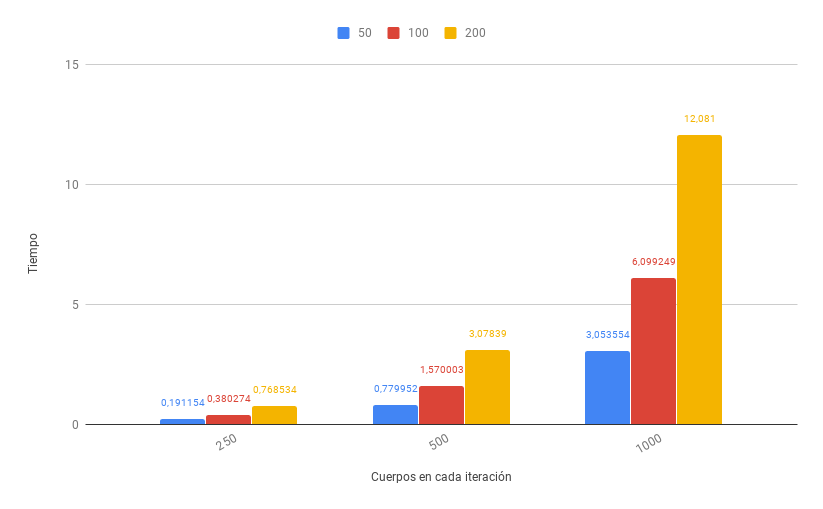
\includegraphics[width=\linewidth]{images/chart.png}
            \end{figure}
        
            \begin{center}
                \noindent Asteroides Iteraciones Planetas $\rightarrow$ Tiempo \\
                250 50 250 $\rightarrow$ 0,175325 s \\
                250 100 250 $\rightarrow$ 0,347015 s \\
                250 200 250 $\rightarrow$ 0,679755 s \\
                500 50 500 $\rightarrow$ 0,684033 s \\
                500 100 500 $\rightarrow$ 1,354324 s \\
                500 200 500 $\rightarrow$ 2,691718 s \\
                1000 50 1000 $\rightarrow$ 2,726185 s \\
                1000 100 1000 $\rightarrow$ 5,425178 s \\
                1000 200 1000 $\rightarrow$ 10,784117 s \\
            \end{center}
            
            \newpage
            \begin{center}
                Tiempo medio por iteración
            \end{center}
            \begin{figure}[hbt!]
                \centering
                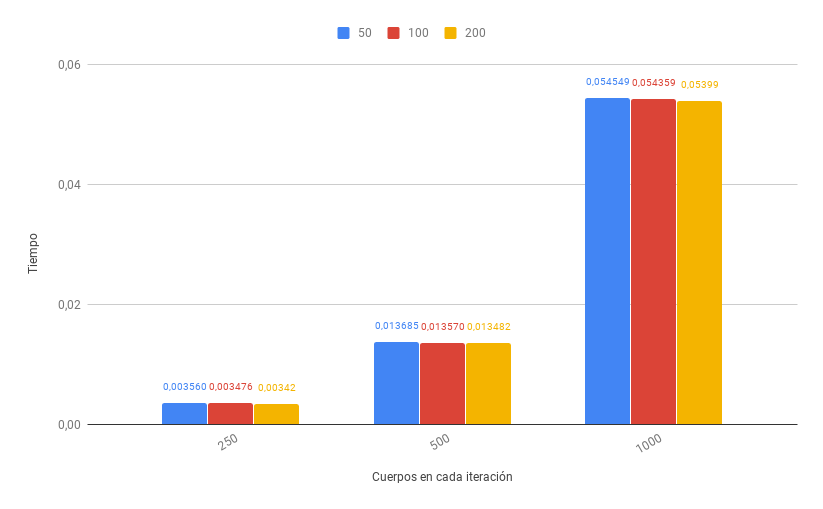
\includegraphics[width=\linewidth]{images/chart2.png}
            \end{figure}
        
            \begin{center}
                \noindent Asteroides Iteraciones Planetas $\rightarrow$ Tiempo \\
                250 50 250 $\rightarrow$ 0,003560 s \\
                250 100 250 $\rightarrow$ 0,003476 s \\
                250 200 250 $\rightarrow$ 0,003420 s \\
                500 50 500 $\rightarrow$ 0,013685 s \\
                500 100 500 $\rightarrow$ 0,013570 s \\
                500 200 500 $\rightarrow$ 0,013482 s \\
                1000 50 1000 $\rightarrow$ 0,054549 s \\
                1000 100 1000 $\rightarrow$ 0,054359 s \\
                1000 200 1000 $\rightarrow$ 0,053990 s \\
            \end{center}
        
        \newpage
        \subsubsection{Análisis de resultados}
    \newpage
    \section{Paralelo}
        \subsection{Introducción}
        \noindent Para realizar esta parte hemos cogido el código secuencial y con la librería OpenMP hemos añadido paralelismo a la hora de escribir (separando parámetros, asteroides y planetas). Además hemos puesto varios hilos en el bucle principal del programa.
        \subsection{Pruebas de rendimiento}
        \subsubsection{Prámetros de la máquina empleada}
            \begin{enumerate}
                \item Procesador $\rightarrow$ AMD Ryzen 5 1600 Six-Core Processor
                \item Núcleos $\rightarrow$ 12
                \item Hilos $\rightarrow$ 24
                \item Memoria Principal $\rightarrow$ 16032 MiB
                \item Memoria Caché:
                    \begin{enumerate}
                        \item L1d $\rightarrow$ 192 KiB
                        \item L1i $\rightarrow$ 384 KiB
                        \item L2 $\rightarrow$ 3 MiB
                        \item L3 $\rightarrow$ 16 MiB
                    \end{enumerate}
                \item Sistema Operativo $\rightarrow$ ArchLabs Linux x86\_64
                \item Versión gcc $\rightarrow$ 9.1.0
            \end{enumerate}
        \newpage
        \subsubsection{Pruebas}
        %%%%%%%%%%%%%%%%%%%%%%%%%%%%%%%%%%%%%%%%%%%%%%%%%%%%%%%%%%%%%
            \begin{enumerate}[label=(\Alph*)]
            \textbf{\item 1 Hilo} \\
                \begin{center}
                    Tiempo medio por ejecución
                \end{center}
                \begin{figure}[hbt!]
                    \centering
                    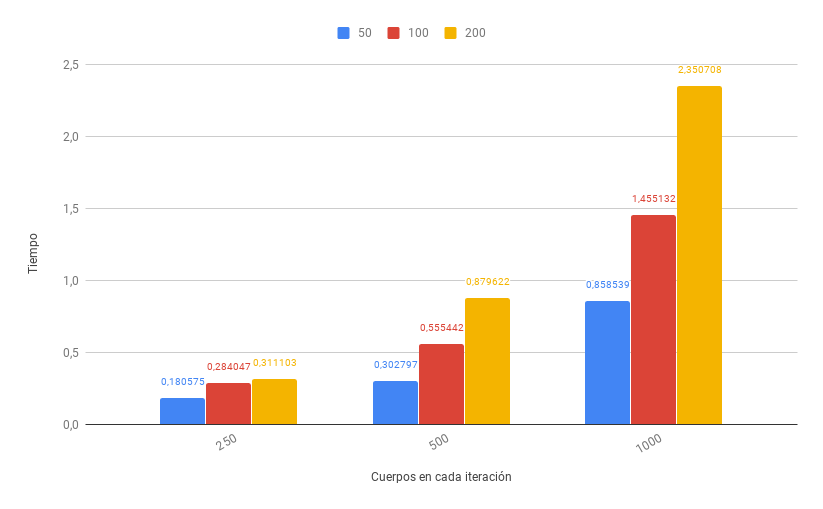
\includegraphics[width=\linewidth]{images/chart3.png}
                \end{figure}
                
                \begin{center}
                    \noindent Asteroides Iteraciones Planetas $\rightarrow$ Tiempo \\
                    250 50 250 $\rightarrow$ 0,180575 s \\
                    250 100 250 $\rightarrow$ 0,284047 s \\
                    250 200 250 $\rightarrow$ 0,311103 s \\
                    500 50 500 $\rightarrow$ 0,302797 s \\
                    500 100 500 $\rightarrow$ 0,555442 s \\
                    500 200 500 $\rightarrow$ 0,879622 s \\
                    1000 50 1000 $\rightarrow$ 0,858539 s \\
                    1000 100 1000 $\rightarrow$ 1,455132 s \\
                    1000 200 1000 $\rightarrow$ 2,350708 s \\
                \end{center}
                
                \newpage
                \begin{center}
                    Tiempo medio por iteración
                \end{center}
                \begin{figure}[hbt!]
                    \centering
                    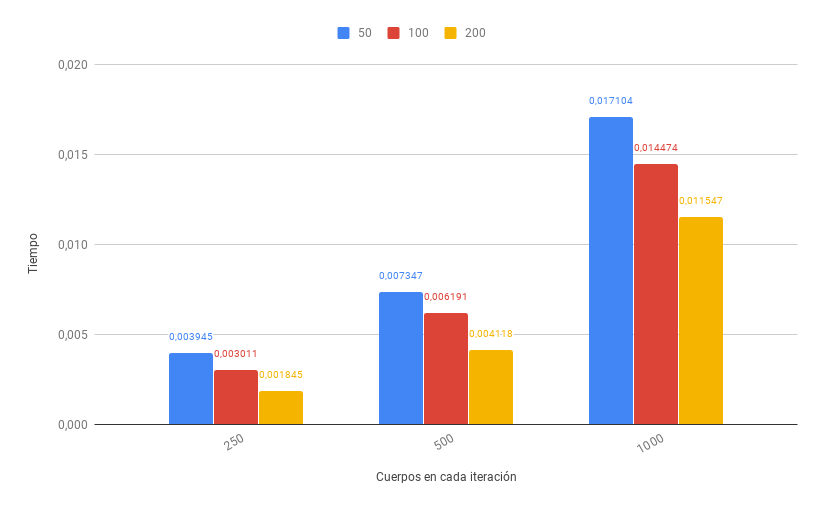
\includegraphics[width=\linewidth]{images/chart4.png}
                \end{figure}
                
                \begin{center}
                    \noindent Asteroides Iteraciones Planetas $\rightarrow$ Tiempo \\
                    250 50 250 $\rightarrow$ 0,003945 s \\
                    250 100 250 $\rightarrow$ 0,003011 s \\
                    250 200 250 $\rightarrow$ 0,001845 s \\
                    500 50 500 $\rightarrow$ 0,007347 s \\
                    500 100 500 $\rightarrow$ 0,006191 s \\
                    500 200 500 $\rightarrow$ 0,004118 s \\
                    1000 50 1000 $\rightarrow$ 0,017104 s \\
                    1000 100 1000 $\rightarrow$ 0,014474 s \\
                    1000 200 1000 $\rightarrow$ 0,011547 s \\
                \end{center}
        %%%%%%%%%%%%%%%%%%%%%%%%%%%%%%%%%%%%%%%%%%%%%%%%%%%%%%%%%%%%%
            \newpage
            \textbf{\item 2 Hilos} \\
                \begin{center}
                    Tiempo medio por ejecución
                \end{center}
                \begin{figure}[hbt!]
                    \centering
                    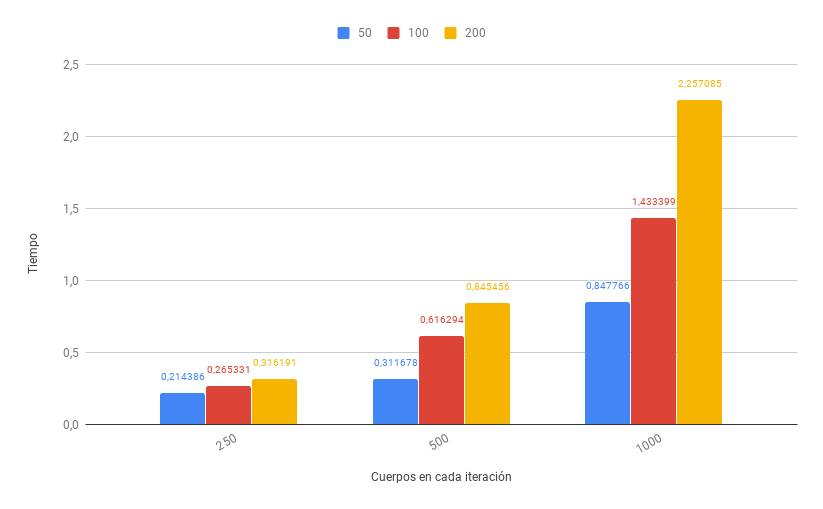
\includegraphics[width=\linewidth]{images/chart5.png}
                \end{figure}
                
                \begin{center}
                    \noindent Asteroides Iteraciones Planetas $\rightarrow$ Tiempo \\
                    250 50 250 $\rightarrow$ 0,214386 s \\
                    250 100 250 $\rightarrow$ 0,265331 s \\
                    250 200 250 $\rightarrow$ 0,316191 s \\
                    500 50 500 $\rightarrow$ 0,311678 s \\
                    500 100 500 $\rightarrow$ 0,616294 s \\
                    500 200 500 $\rightarrow$ 0,845456 s \\
                    1000 50 1000 $\rightarrow$ 0,847766 s \\
                    1000 100 1000 $\rightarrow$ 1,433399 s \\
                    1000 200 1000 $\rightarrow$ 2,257085 s \\
                \end{center}
                
                \newpage
                \begin{center}
                    Tiempo medio por iteración
                \end{center}
                \begin{figure}[hbt!]
                    \centering
                    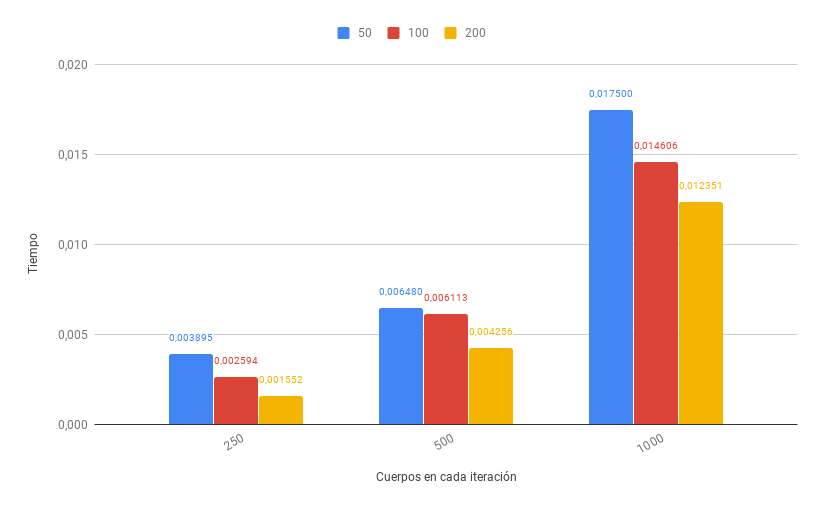
\includegraphics[width=\linewidth]{images/chart6.png}
                \end{figure}
                
                \begin{center}
                    \noindent Asteroides Iteraciones Planetas $\rightarrow$ Tiempo \\
                    250 50 250 $\rightarrow$ 0,003895 s \\
                    250 100 250 $\rightarrow$ 0,002594 s \\
                    250 200 250 $\rightarrow$ 0,001552 s \\
                    500 50 500 $\rightarrow$ 0,006480 s \\
                    500 100 500 $\rightarrow$ 0,006113 s \\
                    500 200 500 $\rightarrow$ 0,004256 s \\
                    1000 50 1000 $\rightarrow$ 0,017500 s \\
                    1000 100 1000 $\rightarrow$ 0,014606 s \\
                    1000 200 1000 $\rightarrow$ 0,012351 s \\
                \end{center}
        %%%%%%%%%%%%%%%%%%%%%%%%%%%%%%%%%%%%%%%%%%%%%%%%%%%%%%%%%%%%%
            \newpage
            \textbf{\item 4 Hilos} \\
                \begin{center}
                    Tiempo medio por ejecución
                \end{center}
                \begin{figure}[hbt!]
                    \centering
                    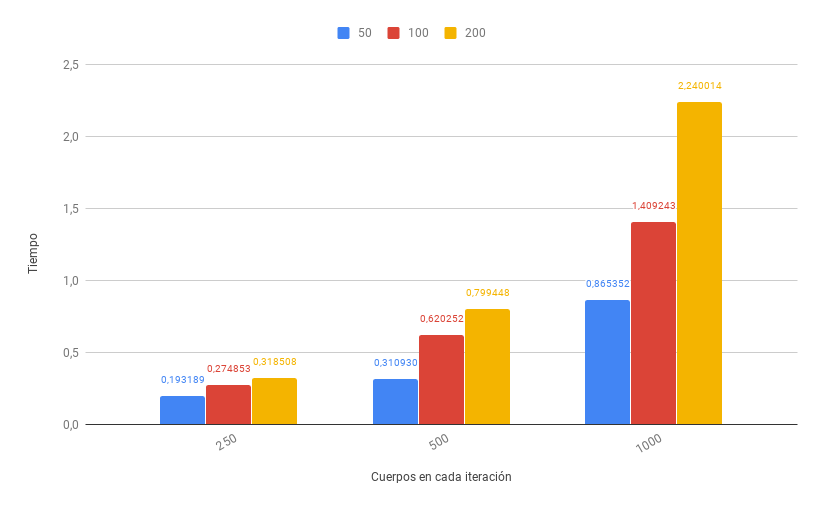
\includegraphics[width=\linewidth]{images/chart7.png}
                \end{figure}
                
                \begin{center}
                    \noindent Asteroides Iteraciones Planetas $\rightarrow$ Tiempo \\
                    250 50 250 $\rightarrow$ 0,193189 s \\
                    250 100 250 $\rightarrow$ 0,274853 s \\
                    250 200 250 $\rightarrow$ 0,318508 s \\
                    500 50 500 $\rightarrow$ 0,310930 s \\
                    500 100 500 $\rightarrow$ 0,620252 s \\
                    500 200 500 $\rightarrow$ 0,799448 s \\
                    1000 50 1000 $\rightarrow$ 0,865352 s \\
                    1000 100 1000 $\rightarrow$ 1,409243 s \\
                    1000 200 1000 $\rightarrow$ 2,240014 s \\
                \end{center}
                
                \newpage
                \begin{center}
                    Tiempo medio por iteración
                \end{center}
                \begin{figure}[hbt!]
                    \centering
                    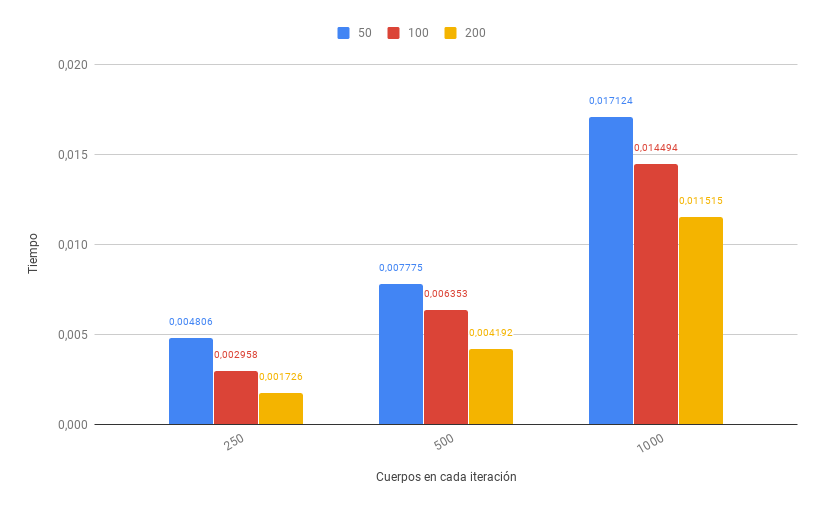
\includegraphics[width=\linewidth]{images/chart8.png}
                \end{figure}
        
                \begin{center}
                    \noindent Asteroides Iteraciones Planetas $\rightarrow$ Tiempo \\
                    250 50 250 $\rightarrow$ 0,004806 s \\
                    250 100 250 $\rightarrow$ 0,002958 s \\
                    250 200 250 $\rightarrow$ 0,001726 s \\
                    500 50 500 $\rightarrow$ 0,007775 s \\
                    500 100 500 $\rightarrow$ 0,006353 s \\
                    500 200 500 $\rightarrow$ 0,004192 s \\
                    1000 50 1000 $\rightarrow$ 0,017124 s \\
                    1000 100 1000 $\rightarrow$ 0,014494 s \\
                    1000 200 1000 $\rightarrow$ 0,011515 s \\
                \end{center}
        %%%%%%%%%%%%%%%%%%%%%%%%%%%%%%%%%%%%%%%%%%%%%%%%%%%%%%%%%%%%%
            \newpage
            \textbf{\item 8 Hilos} \\
                \begin{center}
                    Tiempo medio por ejecución
                \end{center}
                \begin{figure}[hbt!]
                    \centering
                    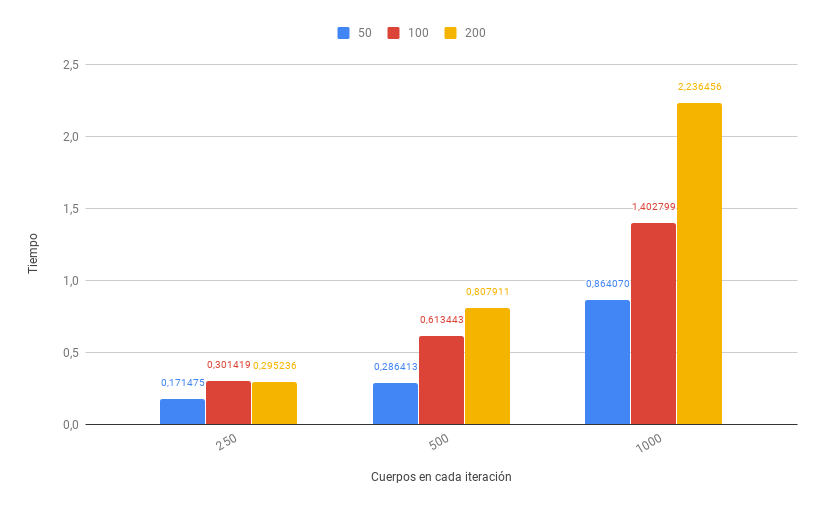
\includegraphics[width=\linewidth]{images/chart9.png}
                \end{figure}
            
                \begin{center}
                    \noindent Asteroides Iteraciones Planetas $\rightarrow$ Tiempo \\
                    250 50 250 $\rightarrow$ 0,171475 s \\
                    250 100 250 $\rightarrow$ 0,301419 s \\
                    250 200 250 $\rightarrow$ 0,295236 s \\
                    500 50 500 $\rightarrow$ 0,286413 s \\
                    500 100 500 $\rightarrow$ 0,613443 s \\
                    500 200 500 $\rightarrow$ 0,807911 s \\
                    1000 50 1000 $\rightarrow$ 0,864070 s \\
                    1000 100 1000 $\rightarrow$ 1,402799 s \\
                    1000 200 1000 $\rightarrow$ 2,236456 s \\
                \end{center}
                
                \newpage
                \begin{center}
                    Tiempo medio por iteración
                \end{center}
                \begin{figure}[hbt!]
                    \centering
                    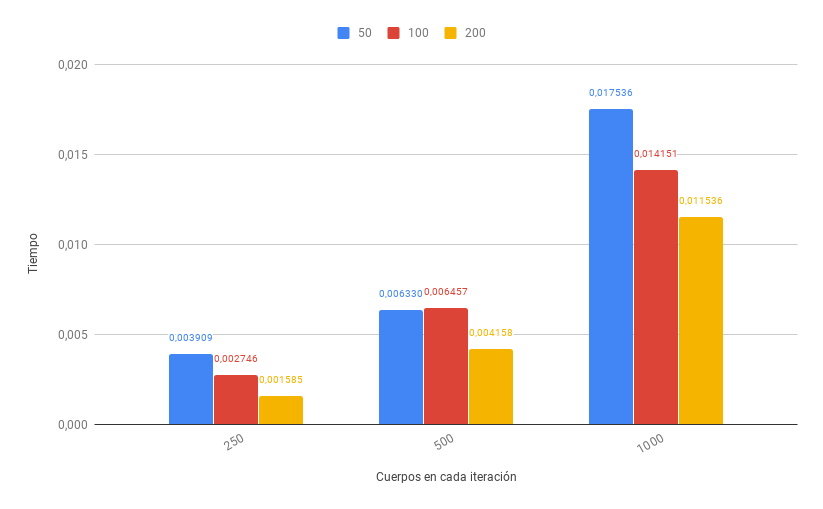
\includegraphics[width=\linewidth]{images/chart10.png}
                \end{figure}
                
                \begin{center}
                    \noindent Asteroides Iteraciones Planetas $\rightarrow$ Tiempo \\
                    250 50 250 $\rightarrow$ 0,003909 s \\
                    250 100 250 $\rightarrow$ 0,002746 s \\
                    250 200 250 $\rightarrow$ 0,001585 s \\
                    500 50 500 $\rightarrow$ 0,006330 s \\
                    500 100 500 $\rightarrow$ 0,006457 s \\
                    500 200 500 $\rightarrow$ 0,004158 s \\
                    1000 50 1000 $\rightarrow$ 0,017536 s \\
                    1000 100 1000 $\rightarrow$ 0,014151 s \\
                    1000 200 1000 $\rightarrow$ 0,011536 s \\
                \end{center}
        %%%%%%%%%%%%%%%%%%%%%%%%%%%%%%%%%%%%%%%%%%%%%%%%%%%%%%%%%%%%%
            \newpage
            \textbf{\item 16 Hilos} \\
                \begin{center}
                    Tiempo medio por ejecución
                \end{center}
                \begin{figure}[hbt!]
                    \centering
                    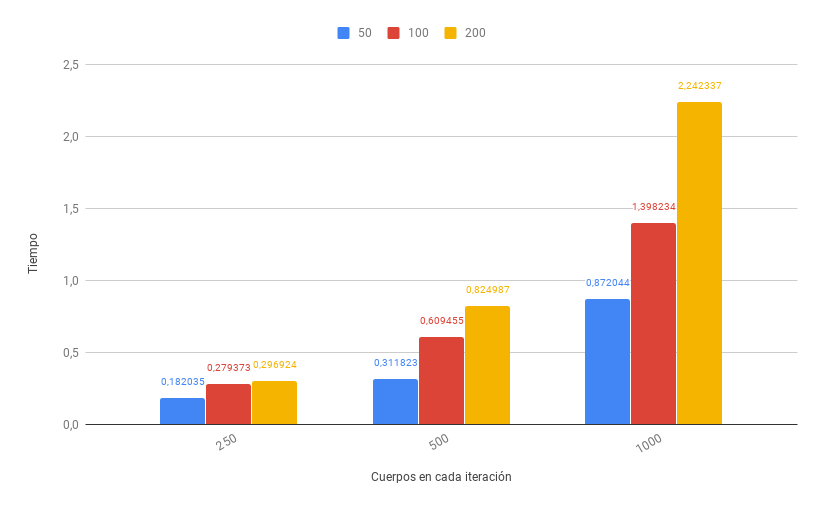
\includegraphics[width=\linewidth]{images/chart11.png}
                \end{figure}
                
                \begin{center}
                    \noindent Asteroides Iteraciones Planetas $\rightarrow$ Tiempo \\
                    250 50 250 $\rightarrow$ 0,182035 s \\
                    250 100 250 $\rightarrow$ 0,279373 s \\
                    250 200 250 $\rightarrow$ 0,296924 s \\
                    500 50 500 $\rightarrow$ 0,311823 s \\
                    500 100 500 $\rightarrow$ 0,609455 s \\
                    500 200 500 $\rightarrow$ 0,824987 s \\
                    1000 50 1000 $\rightarrow$ 0,872044 s \\
                    1000 100 1000 $\rightarrow$ 1,398234 s \\
                    1000 200 1000 $\rightarrow$ 2,242337 s \\
                \end{center}
                
                \newpage
                \begin{center}
                    Tiempo medio por iteración
                \end{center}
                \begin{figure}[hbt!]
                    \centering
                    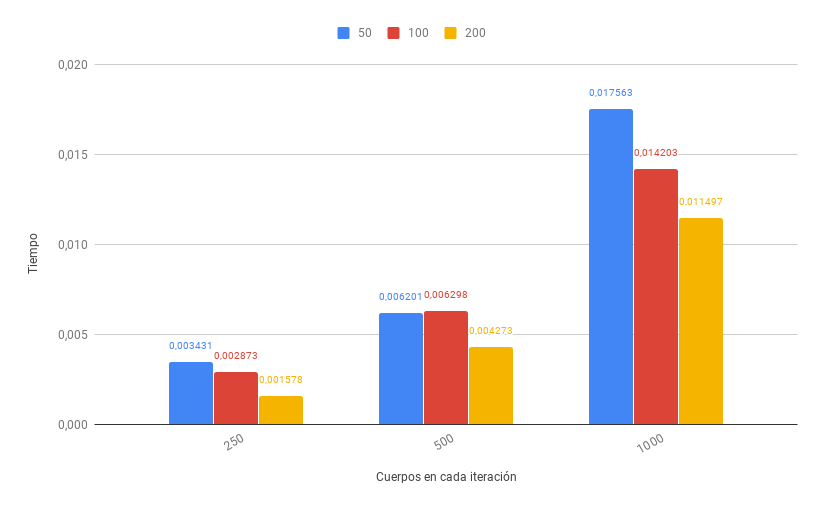
\includegraphics[width=\linewidth]{images/chart12.png}
                \end{figure}
                
                \begin{center}
                    \noindent Asteroides Iteraciones Planetas $\rightarrow$ Tiempo \\
                    250 50 250 $\rightarrow$ 0,003431 s \\
                    250 100 250 $\rightarrow$ 0,002873 s \\
                    250 200 250 $\rightarrow$ 0,001578 s \\
                    500 50 500 $\rightarrow$ 0,006201 s \\
                    500 100 500 $\rightarrow$ 0,006298 s \\
                    500 200 500 $\rightarrow$ 0,004273 s \\
                    1000 50 1000 $\rightarrow$ 0,017563 s \\
                    1000 100 1000 $\rightarrow$ 0,014203 s \\
                    1000 200 1000 $\rightarrow$ 0,011497 s \\
                \end{center}
            \end{enumerate}
        \newpage
        \subsubsection{Análisis de resultados}
        \subsubsection{Impacto de la planificación}
        %Hacer un análisis con las diferencias de:
        %static hilos=4
        %dynamic hilos=4
        %guided hilos=4
        %static hilos=8
        %dynamic hilos=8
        %guided hilos=8
    \newpage
    \section{Conclusión}
    \noindent
%%%%%%%%%%%%%%%%%%%%%%%%%%%%%%%%%%%%%%%%%%%%%%%%%%%%%%%%%%%%%%%%%%%%%%%%%%%%%%%%%%%%%%%%%%%%%%%%%%%%%%%%%%%%%
    %Contraportada
    \newpage
    \blankpage
\end{document}